\documentclass[a4paper,11pt]{book}
\usepackage[francais]{babel}
\usepackage[table]{xcolor}
\usepackage{amsmath}
\usepackage[utf8]{inputenc}
\usepackage{textcomp}
\usepackage{gensymb}
%\usepackage[francais]{babel}
\usepackage[T1]{fontenc}
\usepackage{makeidx}
\usepackage{graphicx}
\usepackage{enumitem}
\usepackage{float}
\usepackage{relsize}
\usepackage{amsmath,amsfonts,amssymb}
\usepackage{multirow}
\usepackage{layout}
\usepackage{amsthm}
\usepackage{lmodern}
\usepackage{fancyhdr}
\usepackage{enumitem}
\usepackage{geometry}
\usepackage{listings}
\usepackage{eso-pic}


\lstdefinestyle{generalFrame}{
aboveskip=3mm,
belowskip=-2mm,
basicstyle=\footnotesize,
breakatwhitespace=false,
breaklines=true,
captionpos=b,
commentstyle=\color{red},
deletekeywords={...},
escapeinside={\%*}{*)},
extendedchars=true,
framexleftmargin=16pt,
framextopmargin=3pt,
framexbottommargin=6pt,
frame=tb,
keepspaces=true,
keywordstyle=\color{blue},
language=Python,
literate=
{²}{{\textsuperscript{2}}}1
{⁴}{{\textsuperscript{4}}}1
{⁶}{{\textsuperscript{6}}}1
{⁸}{{\textsuperscript{8}}}1
{€}{{\euro{}}}1
{é}{{\'e}}1
{è}{{\`{e}}}1
{ê}{{\^{e}}}1
{ë}{{\¨{e}}}1
{É}{{\'{E}}}1
{Ê}{{\^{E}}}1
{û}{{\^{u}}}1
{ù}{{\`{u}}}1
{â}{{\^{a}}}1
{à}{{\`{a}}}1
{á}{{\'{a}}}1
{ã}{{\~{a}}}1
{Á}{{\'{A}}}1
{Â}{{\^{A}}}1
{Ã}{{\~{A}}}1
{ç}{{\c{c}}}1
{Ç}{{\c{C}}}1
{õ}{{\~{o}}}1
{ó}{{\'{o}}}1
{ô}{{\^{o}}}1
{Õ}{{\~{O}}}1
{Ó}{{\'{O}}}1
{Ô}{{\^{O}}}1
{î}{{\^{i}}}1
{Î}{{\^{I}}}1
{í}{{\'{i}}}1
{Í}{{\~{Í}}}1,
morekeywords={*,...},
numbers=none,
numbersep=10pt,
numberstyle=\tiny\color{black},
rulecolor=\color{black},
showspaces=false,
showstringspaces=false,
showtabs=false,
stepnumber=1,
stringstyle=\color{gray},
tabsize=4,
title=\lstname,
}

\definecolor{darkwhite}{rgb}{0.94,0.94,0.94}
\definecolor{darkseagreen}{rgb}{0.56, 0.74, 0.56}
\definecolor{darkpastelblue}{rgb}{0.47, 0.62, 0.8}

\lstnewenvironment{mypython}
  {\lstset{language=Python,
  style =generalFrame,
  backgroundcolor=\color{darkwhite} }}
  {}

\lstnewenvironment{mybash}
  {\lstset{language=bash,
  	style=generalFrame,
	backgroundcolor=\color{darkseagreen} }}
  {}

\lstnewenvironment{myoutput}
  {\lstset{language=bash,
  	style=generalFrame,
	backgroundcolor=\color{darkpastelblue} }}
  {}


\geometry{hmargin=2.2cm,vmargin=2.9cm}

 
\pagestyle{fancy}
\fancyhf{}
\fancyhead[L]{\leftmark}
\fancyfoot[C]{\thepage}
    

\def\entetehpos{-50}
\def\entetevpos{540}

\newcommand{\HRule}{\rule{\linewidth}{0.5mm}}


\newcommand{\blap}[1]{\vbox to 0pt{#1\vss}}
\newcommand\AtUpperLeftCorner[3]{%
\put(\LenToUnit{#1},\LenToUnit{\dimexpr\paperheight-#2}){\blap{#3}}%
}
\newcommand\AtUpperRightCorner[3]{%
\put(\LenToUnit{\dimexpr\paperwidth-#1},\LenToUnit{\dimexpr\paperheight-#2}){\blap{\llap{#3}}}%
}

\setlength{\headheight}{15.35403pt}
\begin{document}
\frontmatter

%==============================
%	PAGE DE GARDE
%==============================

%%%% Ancienne Version (use Package PageDeGarde)
%\let\cleardoublepage\clearpage
%\title{ \usefont{T1}{ptm}{m}{n} Tutoriel TensorFlow}

%\annee{2017-2018}

%\Auteur{IKNI Layachi}{}

%\Encadrant{Pag\'e Vincent}{MCF à l'Université des Antilles}

%	Nouvelle version
\begin{titlepage}
	\AddToShipoutPicture{
		\AtUpperLeftCorner{1.5cm}{1cm}{
\includegraphics[height=3cm]{figures/logo_ua_0.jpg}}
		\AtUpperRightCorner{1.5cm}{1cm}{
\includegraphics[height=3cm]{figures/banniere_lamia.png}}
	}
  \begin{sffamily}
  \begin{center}
	~\\[4cm]

    % Title
    \HRule \\[0.4cm]
    { \huge \bfseries Tutoriel TensorFlow\\[0.4cm] }


    
\includegraphics[width=10cm]{figures/logoTensorFlow.png}
    \HRule \\[6cm]


    % Author and supervisor
	
    \begin{minipage}{0.8\textwidth}
      \begin{flushleft} \large
        IKNI \textsc{Layachi}\\
        PAG\'E \textsc{Vincent}\\
      \end{flushleft}
    \end{minipage}
    \vfill    
    % Bottom of the page
    {\large 1\ier{} janvier 2018}
  \end{center}
  \end{sffamily}
\end{titlepage}
\ClearShipoutPicture

%\maketitle

%\newpage
%\section*{Remerciements}
%\bigskip
%\pagestyle{plain}
%\bigskip
%\newpage 

\newpage
\tableofcontents

\mainmatter
\chapter{Introduction }


\section{Installation}
TensorFlow est une librairie de calcul dédiée à l'apprentissage automatique. On peut l'utiliser avec python, java, C,.... Dans notre cas, nous utiliserons python.


Pour l'installation, nous avons suivi les instructions du tutoriel officiel qui se trouve ici, sans difficultés :

https://www.tensorflow.org/install/

A noter pour les installations de TensorFlow avec virtualEnv (sous Linux), il nous semble raisonnable d'avoir un répertoire contenant les environnements virtuels, dont celui correspondant a TensorFlow (disons \verb+~/VirtualEnvs/TensorFlow+) et un répertoire contenant les sources du projet (disons \verb+~/DNN+).


\section{Présentation TensorFlow et TensorBoard}

\subsection{Premiers concepts de TensorFlow}

Tout d'abord, on peut utiliser TensorFlow de deux façons :
\begin{itemize}
\item En utilisant des algorithmes précodés, utilisant la classe \textbf{Estimator}
\item En maitrisant chaque étape du calcul.
\end{itemize}

Dans le second cas, il est nécessaire de comprendre que TensorFlow
s'appuie sur des concepts de programmation très différents d'une programmation standard python.

Pour bien comprendre ces concepts, prenons un exemple :
On veut que notre programme prenne une valeur réelle (x), calcule une valeur  $y = W*x+b$ avec $W$ et $b$ des valeurs réelles que notre programme sera appelé à modifier plus tard.

Le code correspondant en python est le suivant
\begin{mypython}
x = 2
W = 0.3
b = -0.3
y = W*x+b
print(y)
\end{mypython}

La sortie de ce programme serait :
\begin{myoutput}
0.3
\end{myoutput}

ici, $W$, $b$ , $x$ et $y$ sont des variables du programmes.
Néanmoins, dans le contexte de notre programme, elles jouent des rôles très différents :
\begin{itemize}
\item $x$ est une entrée 
\item $W$ et $b$ sont des valeurs modifiables
\item $y$ est calculé à partir de $x$, $W$ et $b$
\end{itemize}

La programmation en TensorFlow, met en place cette différence.
\begin{itemize}
\item $x$ sera appelé un \textbf{placeholder} , (en deux mots : une variable dont on promet qu'on lui donnera une valeur au moment du run)
\item $W$ et $b$ seront définis comme des variables
\item $y$ sera défini implicitement par l'équation de calcul 
\end{itemize}

Notons qu'il existe aussi la notion de constante, non présentée ici, mais facile a appréhender.

Le code correspondant en TensorFlow est le suivant :
\begin{mypython}
import tensorflow as tf

x = tf.placeholder(tf.float32)

W = tf.Variable([.3], dtype=tf.float32)
b = tf.Variable([-.3], dtype=tf.float32)

y = W*x + b

print(y)
\end{mypython}

La sortie de ce programme est alors surprenante :
\begin{myoutput}
Tensor("add:0", dtype=float32)
\end{myoutput}

De fait, nous n'avons pas calculé la valeur de $y$.\\
En fait notre programme ne manipule pas des variables au sens traditionnel, mais explique les dépendances entres les différents éléments de notre programme (ce sont des nœuds du graphes de calcul). TensorFlow s'appuie sur ce graphe de calcul, sur lequel nous reviendrons plus tard pour comprendre son intérêt.\\

Le graphe correspondant est représenté ci-dessous pour information.
\begin{figure}[H]

\begin{center}
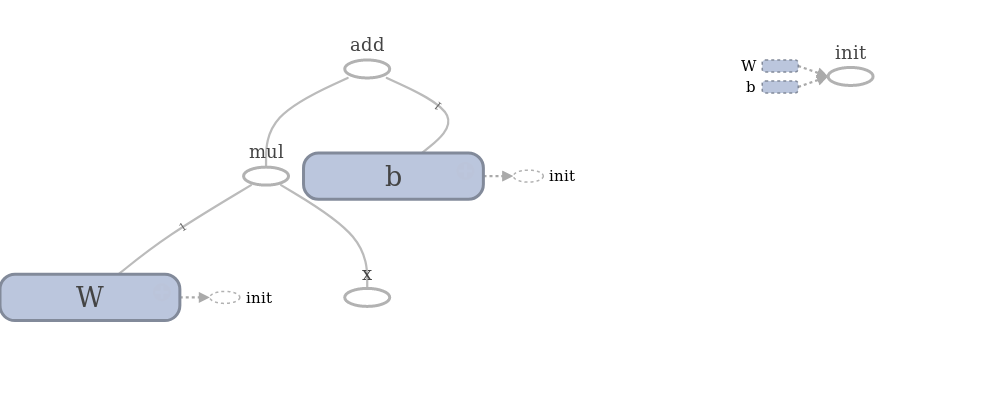
\includegraphics[width=10cm]{./figures/graphAddition.png} 
\end{center}
\caption{Graphe de calcul simple}
\end{figure}

On retrouve dans ce graphes la présence des deux variables ($W$ et $b$), le placeholder $x$, et un noeud $add$ dont la sortie correspond à $y$.


Par ailleurs, les variables au sens TensorFlow sont des nœuds de calculs qui peuvent être modifiés. Elle ne sont pas initialisées par leur déclaration. Il faudra explicitement demander leur initialisation pour qu'elles agissent comme on s'y attend.
Il s'agit maintenant pour que notre programme calcule bien la valeur voulue de :
\begin{itemize}
\item construire le graphe de calcul a partir des informations précédentes.
\item initialiser les variables $W$ et $b$
\item lancer le calcul de y avec une valeur choisie pour $x$...
\end{itemize}

Ajoutons les codes suivants à notre programme
\begin{mypython}
sess = tf.Session()
\end{mypython}
Le code ci-dessus construit le graphe.
\begin{mypython}
init = tf.global_variables_initializer()
sess.run(init)
\end{mypython}
Le code ci-dessus initialise toutes les variables du programme (W et b). En fait, ce code construit un noeud de calcul correspondant a l'initialisation (première ligne) et lance le calcul correspondant (deuxième ligne).

\begin{mypython} 
resu = sess.run(y, {x:2}) 
print(resu)
\end{mypython}
Ce code lance le calcul de y, en prenant soin de placer la valeur 2 dans le placeholder x et afficher le résultat attendu
\begin{myoutput}
[0.3]
\end{myoutput}
Pour comprendre l'intérêt de ces concepts de graphe de calcul, ajoutons à la fin de notre programme existant le code suivant :

\begin{mypython} 
resu = sess.run(y, {x:[1, 2, 3]}) 
print(resu)
\end{mypython} 

Cette fois ci, les sorties sont :

\begin{mypython} 
[0.3]
[0.  0.3 0.6]
\end{mypython} 

Nous avons en fait lancé deux runs (deux calculs de y). La première fois, x est un réel, la seconde fois x est un tableau de réels. Dans le second cas, pour chaque valeur de x, une valeur est calculée pour y.
Notre programme a donc mis en place une procédure de calcul (le graphe de calcul) que l'on peut utiliser de multiples fois, avec différentes valeurs d'entrées (qui de plus prennent des formes différentes).

Une grande partie de la force de TensorFlow tient dans ces notions.

Voici donc le code du programme complet. Ce code est contenu dans le fichier :\\
\verb+DNN/Documentation/TutosPython/PremiersCalculs/calculTensorFlow.py+

\lstinputlisting[style=generalFrame,backgroundcolor=\color{darkwhite}]{../../TutosPython/PremiersCalculs/calculTensorFlow.py}

\subsubsection{Formalisation des concepts}
Ceci tient en quelques mots :
\begin{itemize}
\item TensorFlow s'appuie sur un \textbf{graphe de calcul}.
\item Les nœuds de ce graphe sont des \textbf{opérations}.
\item Sur les arêtes de ce graphe circulent des \textbf{tenseurs}. Ces tenseurs sont les sorties des nœuds du graphe.
\item Faire des calculs avec TensorFlow, c'est lancer un run en demandant le calcul d'une de ces sorties.
\end{itemize}

\subsection{Premiers pas avec Tensorboard}

TensorBoard est l'outil de visualisation associé à TensorFlow. Il permet de visualiser le graphe de calcul, mais aussi des valeurs importantes retenues lors des calculs exécutés sur ce graphe de calcul.

Pour sélectionner les informations a visualiser, nous l'indiquerons a notre programme TensorFlow. Le programme sauvegardera ces informations dans un répertoire spécifique.

On pourra alors lancer l'exécutable TensorBoard qui va analyser ce répertoire, créer un serveur web local que l'on pourra consulter pour visualiser nos informations...
Voyons comment tout ceci se fait.


Ajout de code dans le programme TensorFlow (a la fin du programme précédent) :
\begin{mypython}
pathLog="./SaveHere/";
writer = tf.summary.FileWriter(pathLog, sess.graph)
writer.close()
\end{mypython}
Ici, on choisit le répertoire (répertoire de Log) dans lequel seront stockées les informations importantes, et on crée un objet permettant d'écrire les informations de notre programme sur le disque. Ici, nous ne sauvons que le graphe de calcul. Enfin, on ferme cet objet.

Le code du programme complet est contenu dans le fichier :\\
\verb+DNN/Documentation/TutosPython/PremiersCalculs/calculTensorFlowWithTensorBoard.py+

\lstinputlisting[style=generalFrame,backgroundcolor=\color{darkwhite}]{../../TutosPython/PremiersCalculs/calculTensorFlowWithTensorBoard.py}



On lance notre programme TensorFlow 
\begin{mybash}
python .\calculTensorFlowWithTensorBoard.py
\end{mybash}
On lance ensuite TensorBoard sur le répertoire de Log avec la ligne suivante :

\begin{mybash}
tensorboard --logdir=./SaveHere
\end{mybash}


L’exécution donne le message suivant :
\begin{myoutput}
Starting TensorBoard b'41' on port 6006
(You can navigate to http://127.0.1.1:6006)
\end{myoutput}


Enfin, on ouvre un navigateur dans lequel on indique l'URL de consultation indiquée par la sortie précédente.

Voici une capture de la visualisation obtenue :
\begin{figure}[H]

\begin{center}
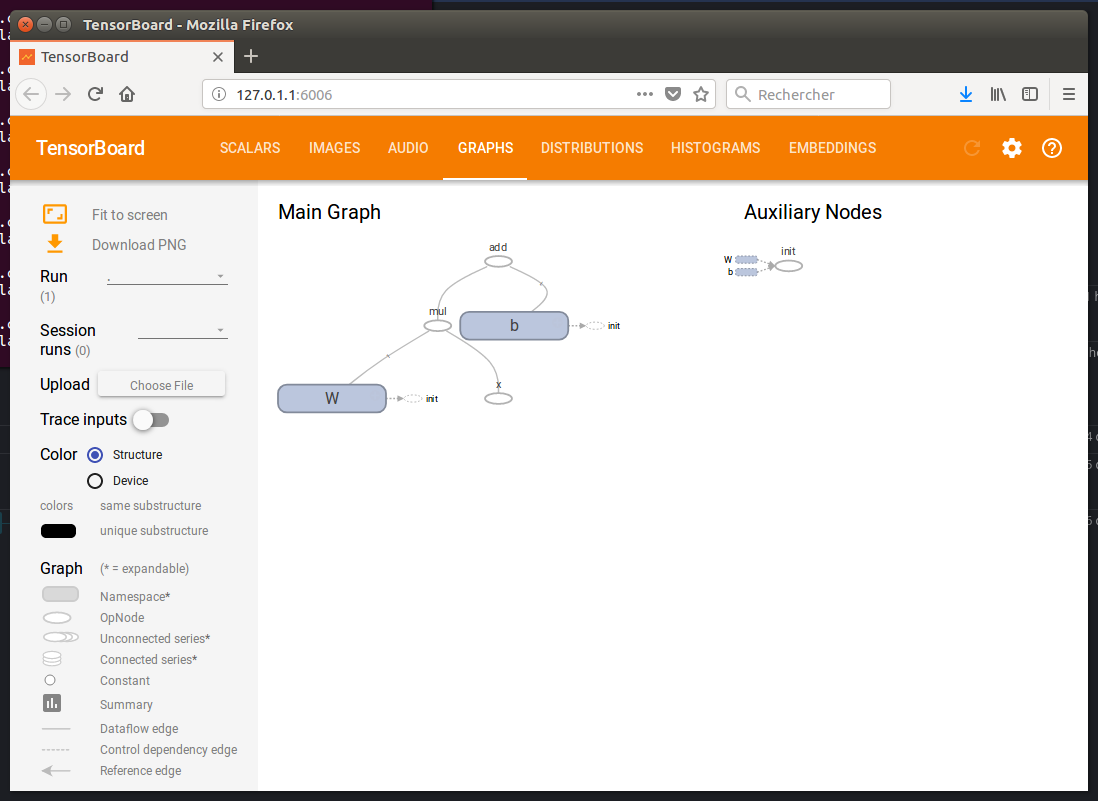
\includegraphics[width=10cm]{./figures/premierTensorBoard.png} 
\end{center}
\caption{La fenêtre de visualisation de TensorBoard}
\end{figure}

On retrouve ici le graphe précédent. Notez le sous graphe en haut a droite (noeud init) correspondant à l'initialisation des variables dont nous avons parlé précédemment.
On verra plus loin que TensorBoard nous permet aussi de visualiser l'évolution de nos apprentissages...

\chapter{Première Classification : Base IRIS}

Sur cette base comme pour les autres, nous allons considérer deux cas :
\begin{itemize}
\item on crée le classifieur manuellement (boite blanche)
\item on utilise un classifieur prédéfini (boite noire)
\end{itemize}

Pour chaque classifieur, nous sauverons le modèle après l'apprentissage, et le rechargerons pour les prédictions.

\section{La Base Iris}

l' ensemble de données Iris est utilisé pour prédire les espèces de fleurs basées sur la géométrie des sépales / pétales. Pour cet exemple  les données Iris ont été randomisées et divisées en deux CSV distincts:
\begin {itemize}
\item Un ensemble d'apprentissage de 120 échantillons ( \verb+iris_training.csv+ )
\item	Un ensemble de test de 30 échantillons ( \verb+iris_test.csv+ ).
\end{itemize}

Cette base a 3 classes possibles et chaque exemple présente 4 caractéristiques.

\section{Réseau monocouche boite blanche}
Le code complet de ce programme sera donné en fin de section. Voyons quelques grandes étapes.

\subsection{lecture des données}
\label{sec:irisMonocoucheRead}
Supposons que les données soient déja présentes sur le disque, on les lira comme suit, par exemple pour la base d'apprentissage.

\begin{mypython}
# Load datasets.
training_set = tf.contrib.learn.datasets.base.load_csv_with_header(
  filename="iris_training.csv",
  target_dtype=np.int,
  features_dtype=np.float32)
\end{mypython}

L'objet \verb+training_set+ a un champ \verb+data+ qui contient les paramètres des exemples et un champ \verb+ target+ qui contient les labels des classes.

\subsection{Construction du réseau}
\label{sec:irisMonocoucheBuild}
\subsubsection{Les entrées}
On crée ensuite les placeholders pour entrer ces données:
X est bien de taille 4.  
\begin{mypython}
with tf.name_scope('X'):
	# entrées
	x = tf.placeholder(tf.float32, [None, 4], name = "X")

with tf.name_scope('Y_True'):
    # sorties voulues
    y_int = tf.placeholder(tf.uint8, [None], name = "Y_int")
    y_ = tf.one_hot(y_int, depth=3, name = "Y_True")

\end{mypython}
A noter que l'on crée ici un noeud \verb+y_+ qui transforme le label (entier) d'une classe en un \textbf{hot vector}.
Par exemple, le label 0 parmi 3 classes possibles se transforme en hot vecteur : \verb+[1,0,0]+\\

\subsubsection{Le modèle}
Définissons notre modèle : un réseau monocouche linéaire.
Nous avons 3 neurones de sortie (1 par classe).
Chaque neurone a 4 entrées (les 4 paramètres).
Nous avons 4 poids et 1 biais par neurone.
Le score calculé pour chaque classe est classique.
\begin{mypython}
# Le modèle
with tf.name_scope("Weights"):
	W = tf.Variable(tf.zeros([4, 3]),name ="W")

with tf.name_scope("Biases"):
	b = tf.Variable(tf.zeros([3]), name = "b")
	
with tf.name_scope("Score"):
	score = tf.matmul(x, W) + b
\end{mypython}
Les lignes de type \verb+with tf.name_scope("Score"):+ servent juste à regrouper certains nœuds pour la visualisation avec TensorBoard.

\subsubsection{optimisation du modèle}
Pour trouver les meilleurs poids $(W,b)$ du réseau, il nous faut : un critère à minimiser, et un algorithme de minimisation.


Le critère à minimiser sera pour nous \textbf{l'entropie croisée}.
Pour le calculer, nous transformons les scores de chaque sortie en une probabilité (fonction \verb+softmax+). On veut ensuite calculer une distance entre ce vecteur de probabilité et la distribution voulue (le hot vector d'entrée). L'entropie croisée fera office de distance.
\begin{mypython}
with tf.name_scope('softmax'):
	y = tf.nn.softmax(score)
with tf.name_scope('cross_entropy'):
	cross_entropy = tf.reduce_mean(-tf.reduce_sum(y_ * tf.log(y), reduction_indices=[1]))
\end{mypython}

Pour savoir quelle est la classe prédite il faut regarder quelle sortie a donné le plus fort score :
\begin{mypython}
classe = tf.argmax(y,1)    
\end{mypython}

Pour mesurer la précision (le taux de reconnaissance), il faut vérifier si la classe retenue pour un exemple est bien la classe donnée par la base. On calcule ensuite le taux moyen de succès sur un ensemble d'exemples :
\begin{mypython}
with tf.name_scope('Accuracy'):
	correct_prediction = tf.equal(tf.argmax(y,1), tf.argmax(y_,1))
	accuracy = tf.reduce_mean(tf.cast(correct_prediction, tf.float32))
\end{mypython}

On choisit enfin une méthode d'optimisation. Ici, une descente de gradient appliquée à notre entropie croisée.
\begin{mypython}
# Choix d'une méthode de minimisation
with tf.name_scope('train'):
	train_step = tf.train.GradientDescentOptimizer(0.5).minimize(cross_entropy)
\end{mypython}
Cette descente de gradient définit un nœud de calcul \verb+train_step+ que l'on pourra appeler lors du run.

\subsection{lancement des calculs}
On initialise tout d'abord les variables du réseau.
\begin{mypython}
init = tf.global_variables_initializer();
sess.run(init);
\end{mypython}

Apprentissage : On lance le run sur le noeud de calcul \verb+train_step+.
\begin{mypython}
for i in range(1000):
  sess.run(train_step, feed_dict={x: training_set.data, y_int: training_set.target})
\end{mypython}

Evaluons notre apprentissage sur la base d'apprentissage : On lance le run sur le noeud de calcul correspondant à la précision. 
\begin{mypython}
print("Resultats en Apprentissage", sess.run(accuracy, feed_dict={x: training_set.data, y_int: training_set.target}))
\end{mypython}

Voyons une prédiction : on lance le run sur le noeud de calcul de classe, avec des exemples inconnus.
\begin{mypython}
new_samples = np.array(
  [[6.9, 3.2, 4.5, 1.5],
   [4.8, 3.1, 5.0, 1.7]], dtype=np.float32)
  
print("classe ", sess.run(classe, {x: new_samples}))
\end{mypython}

A ce stade, nous avons un classifieur fonctionnel.
Ajoutons quelques améliorations pour la visualisation avec TensorBoard.

\subsection{TensorBoard : Evolution des performances}
\label{sec:irisMonocoucheTensorBoard}
Nous allons modifier notre code pour disposer de graphiques d'évolution de la précision et de l'entropie croisée au cours de l'apprentissage.

Commençons par choisir un répertoire, et ouvrons un \verb+FileWriter+ pour écrire dedans
\begin{mypython}
visuPath = './VisuMonoCouche'
writer = tf.summary.FileWriter(visuPath, sess.graph)
\end{mypython}

Signalons ensuite que nous voulons suivre l'entropie croisée et la précision. Ces infos seront fusionnées pour le \verb+FileWriter+ en un nœud \verb+merged+.
\begin{mypython}
tf.summary.scalar('Entropie Croisee', cross_entropy)
tf.summary.scalar('Precision', accuracy)

merged = tf.summary.merge_all()
\end{mypython}

L'apprentissage doit etre un peu modifié : Quand on lance un run d'apprentissage, on calcule aussi le noeud \verb+merged+. Sa sortie est récupérée dans la variable \verb+summary+. Celle ci est passée au \verb+FileWriter+ qui gère la sauvegarde.
\begin{mypython}
for i in range(1000):
  summary, _ = sess.run([merged,train_step], feed_dict={x: training_set.data, y_int: training_set.target})

  writer.add_summary(summary, i)
\end{mypython}

Ce code permet d'obtenir des visualisations telles que celle ci :
\begin{figure}[H]
\begin{center}
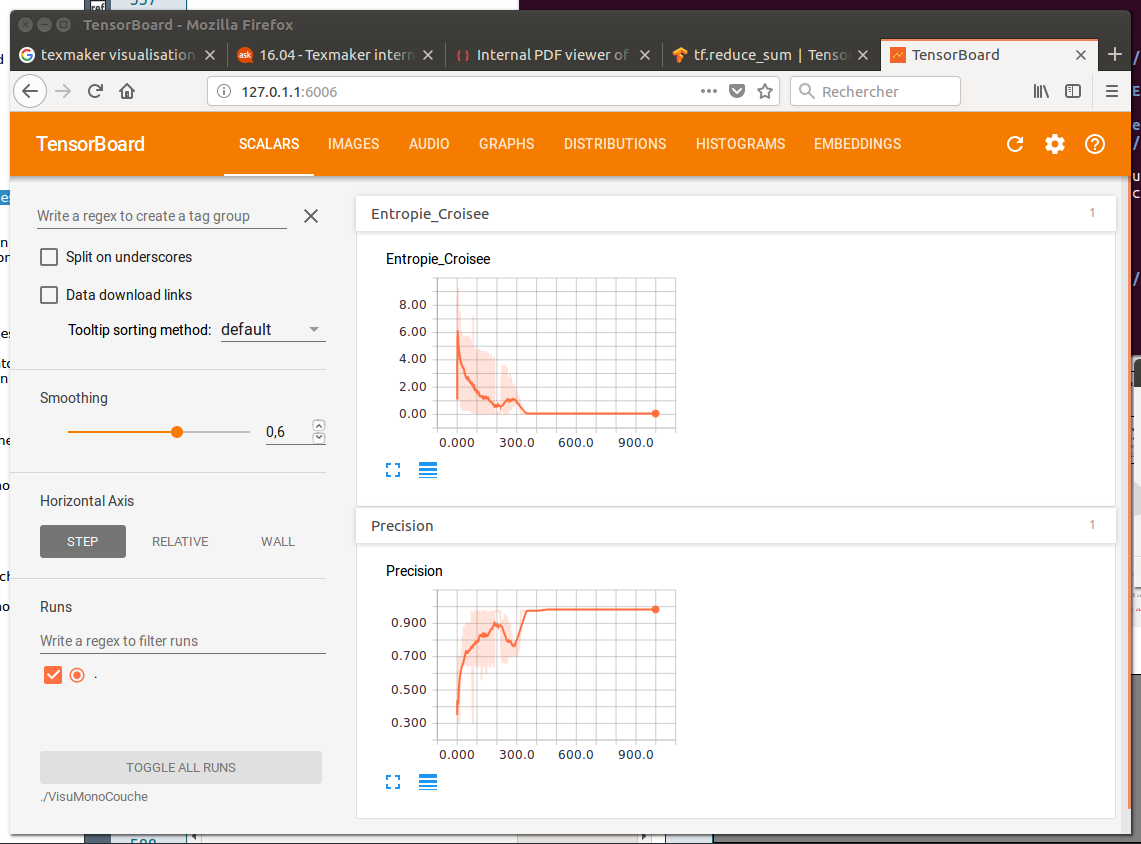
\includegraphics[width=12cm]{./figures/scalarIrisMono.png} 
\end{center}
\caption{Évolution des performances en apprentissage}
\end{figure}

\subsection{Code du programme complet}
On peut améliorer un peu notre programme en téléchargeant la base IRIS si on ne l'a pas sur le disque, et effacer le répertoire de visualisation pour éviter qu'il ne se remplisse de données, ce qui donnerait le programme complet suivant contenu dans le fichier :\\
\verb+DNN/Documentation/TutosPython/Iris/irisMonocoucheComplet.py+

\lstinputlisting[style=generalFrame,backgroundcolor=\color{darkwhite}]{../../TutosPython/Iris/irisMonocoucheComplet.py}

\subsection{Sauvegarde et Chargement d'un réseau }
\label{sec:irisMonocoucheSave}
Il s'agit maintenant de séparer notre programme en deux :
\begin{itemize}
\item Un programme qui apprend, évalue les performances et sauve le réseau
\item Un programme qui charge un réseau entraîné, et fait des prédictions.
\end{itemize}

\subsubsection{Sauvegarde}
La sauvegarde sera prise en charge par l'objet \verb+train.Saver+, qui va sauver le graphe, les variables du graphes (et d'autres choses plus nébuleuses pour les rédacteurs) dans un répertoire.
L'essentiel du code qui fait cela est le suivant.
\begin{mypython}
saver = tf.train.Saver()

savePath = './SavedNetworks/myMonoCouchemodel.ckpt'

saver.save(sess, savePathFull)  
\end{mypython}
Ceci va générer :
\begin{itemize}
\item un fichier \verb+myMonoCouchemodel.ckpt.meta+ qui contient l'architecture du réseau.
\item un fichier \verb+myMonoCouchemodel.ckpt.data-00000-of-00001+ qui contient les valeurs des variables du réseau à l'instant de sauvegarde.
\item un fichier \verb+myMonoCouchemodel.ckpt.index+ qui, je crois, contient le nom des noeuds du réseau.
\item un fichier \verb+checkpoint+ utile mais sans qu'on sache trop pourquoi.
\end{itemize}

\subsubsection{Chargement}
le chargement n'est pas trop compliqué non plus :
\begin{itemize}
\item on charge le fichier d'architecture, ce qui crée le graphe.
\item on recharge l'état du réseau dans le graphe.
\item on récupère les noeuds du graphe qui nous intéressent.
\end{itemize}
\begin{mypython}

sess = tf.Session()

new_saver = tf.train.import_meta_graph('./SavedNetworks/myMonoCouchemodel.ckpt')
  
new_saver.restore(sess, tf.train.latest_checkpoint('./SavedNetworks/))
\end{mypython}
A ce stade, nous disposons d'un réseau pré-entraîné.
Notre programme doit donc lui injecter des données et récupérer certaines sorties. Commencons par obtenir du graphe des pointeurs sur tous ces nœuds d'intérêt.


Lorsque le réseau a été construit lors de l'apprentissage, nous avons crée par exemple le nœud qui calcule la classe comme suit :
\begin{mypython}
with tf.name_scope('Classe'):
    classe = tf.argmax(y,1, name="classe")
\end{mypython}

Le nom complet de ce noeud dans le graphe est "Classe/classe:0". "Classe" pour le nameScope s'il y en a un. "classe" correspond le nom du nœud. ":0" est un indice systématiquement ajouté et auto-incrémenté pour éviter les déclarations multiples accidentelles.

Pour une prédiction, nous devons obtenir des pointeurs sur le placeholder x et sur le nœud des classes :

\begin{mypython}
graph = tf.get_default_graph()

x = graph.get_tensor_by_name("X/X:0")
  
classe = graph.get_tensor_by_name("Classe/classe:0")
\end{mypython}
Il suffit ensuite de lui fournir normalement les exemples pour obtenir les classes.

\begin{mypython}

new_samples = np.array(
    [[5.2, 1.2, 4.5, 1.5],
    [4.8, 6.4, 5.0, 1.7],
    [3.5, 3.2, 2.5, 8.5]], dtype=np.float32)

predictions = sess.run(classe, {x: new_samples})
\end{mypython}

\subsection{Programmes de sauvegarde et prédiction complets}
Dans ces programmes, nous avons ajouté quelques lignes pour paramétrer proprement les noms des fichiers et répertoires de sauvegarde et une procédure qui efface les répertoires de sauvegarde des modèles s'ils existent.

Voici le code du programme qui réalise l'apprentissage, contenu dans le fichier :\\
\verb+DNN/Documentation/TutosPython/Iris/irisMonocoucheTrain.py+

\lstinputlisting[style=generalFrame,backgroundcolor=\color{darkwhite}]{../../TutosPython/Iris/irisMonocoucheTrain.py}


Voici le code du programme qui réalise les prédictions, contenu dans le fichier :\\
\verb+DNN/Documentation/TutosPython/Iris/irisMonocouchePredict.py+

\lstinputlisting[style=generalFrame,backgroundcolor=\color{darkwhite}]{../../TutosPython/Iris/irisMonocouchePredict.py}


\subsection{Quelques remarques sur l'implémentation}
Le lecteur soucieux de faire fonctionner ses programmes pourra sans risque sauter cette section pour revenir dessus quand il aura mieux pris en main TensorFlow.


TensorFlow travaille avec des tenseurs (des tableaux multi-dimensionnels).
Il est intéressant de comprendre quelles tailles ont ces tenseurs dans notre programme.

Dans tous nos programmes, les données insérées dans notre réseau seront de type \verb+NdArray+ de la librairie \verb+numpy+. Leur taille doit correspondre aux placeholders du réseau. Par exemple :
\begin{itemize}
\item \verb+training_set.data+ est un NdArray de dimension 2, de taille (120,4)
\item \verb+training_set.data+ est un NdArray de dimension 1, de taille (120) 
\end{itemize}

Les placeholders ont les caractéristiques suivantes
\begin{itemize}
\item \verb+x+ a pour taille (None,4) : il accepte autant d'exemples que fournis, tous de 4 caractéristiques, chacune en float32.
\item \verb+Y_+ (les labels) a pour taille (None) : il accepte autant de labels que fournis, tous d'une seule valeur entiere.
\end{itemize}

Il faut bien comprendre que le calcul de toutes les sorties pour toutes les entrées se fait en une seule opération. Voyons donc le détail de ceci.

la matrice des poids $W$ est un tenseur de dimension 2, de taille (4,3).

le réseau calcule $tf.matmul(x,W)$ : Le résultat de cette opération est, dans le cas d'un seul exemple, un tenseur de dimension 2, de taille (1, 3)

On lui ajoute le biais $b$, qui est un tenseur de dimension 1, de taille 3.
Le résultat est toujours un tenseur de dimension 1, de taille 3 représentant chaque le score en sortie du réseau pour l'exemple proposé.

Dans le cas ou l'on présente 120 exemples:

Le résultat de $tf.matmul(x,W)$ est un tenseur de dimension 2, de taille (120, 3).

On lui ajoute le tenseur de biais, de dimension 1, et de taille 3. La réussite opérationnelle de cette opération est intéressante \footnote{ Elle est due au concept de broadcasting. voir https://docs.scipy.org/doc/numpy/user/basics.broadcasting.html }

A partir de ces scores, on calcule les probabilités $y$, qui sont toujours un tenseur d'ordre 2, de taille (120, 3)

\verb+y_+, le hot vector correspondant aux labels est lui aussi un tenseur d'ordre 2, de taille (120,3).

La multiplication impliquée dans le calcul de l'entropie croisée est une multiplication point à point.

\verb+tf.reduce_sum+ doit calculer l'entropie pour un exemple. Il opère bien sur la direction 1 (il somme les 3 sorties). Sa sortie est un tenseur d'ordre 1 de taille (120).

\verb+tf.reduce_mean+ doit calculer la moyenne de ces entropies sur tous les exemples. Le tenseur qu'on lui fournit en entrée etant d'ordre 1, il n'y a pas besoin de spécifier de direction pour cette opération.Sa sortie est un tenseur d'ordre 1 de taille (1).


\section{Réseau multi couche Boite Noire }
Dans cette section, nous reprenons tout ce qui a été fait précédemment, en modifiant le modèle, et en utilisant un réseau pré-codé, intégré dans la classe Estimator.

Ce réseau est de type DNN, nous le créerons avec seulement 3 couches.

la classe Estimator dont hérite notre réseau encapsule la plupart des opérations et donne un code beaucoup plus classique, tout le graphe étant masqué. 

\subsection{lecture des données}
Rien de changé, le lecteur peut se référer à la
section~\ref{sec:irisMonocoucheRead}.

\subsection{Construction du réseau}
\label{sec:irisMulticoucheBuild}
\begin{mypython}
feature_columns = [tf.feature_column.numeric_column("x", shape=[4])]
\end{mypython}
Ce code prépare une variable pour les entrées du modèle (le vecteur de caractéristiques ou \textbf{feature vector}) et spécifie que \textbf{feature vector} est numérique et de dimension 4 (longueur des sépales, largeurs des sépales, longueur des pétales, largeur des pétales).

\begin{mypython}
classifier = tf.estimator.DNNClassifier(feature_columns=feature_columns,
                                          hidden_units=[10, 20, 10],
                                          n_classes=3,
                                          model_dir="/VisuDnn")
\end{mypython}
Ce code crée un Réseau de Neurones Profond (Deep Neural Network ou \textbf{DNN}) que l'on utilisera pour classifier nos données. Pour le construire on lui passe les informations suivantes :
\begin{itemize}
\item la forme du \textbf{feature vector}.
\item la topologie du réseau. Ici : trois couches cachées , contenant respectivement 10, 20 et 10 neurones.
\item le nombre de classes attendues en sortie. Ici : Trois classes, représentant les trois espèces d'Iris.
\item le répertoire dans lequel TensorFlow sauvegardera en particulier les données utilisées par  TensorBoard pour la visualisation.
\end{itemize}

\subsection{Lancement des calculs}
La classe Estimator propose trois grandes actions lors d'un apprentissage :
\begin{itemize}
\item Train : on entraine le réseau
\item Evaluate : on évalue le réseau sur une base
\item Predict : on effectue des prédictions sur de nouveaux exemples.
\end{itemize}

Voyons par exemple comment lancer l'apprentissage. la classe Estimator. impose la structure de code suivante :
\begin{itemize}
	\item on définit une fonction spécifiant :
	\begin{itemize}	
		\item le jeu de donnée utilisé (caractéristiques et labels).
		\item le nombre d'\textbf{epochs} lors de l'apprentissage.
		\item si les données doivent être présentées dans un ordre aléatoire
	\end{itemize}
	\item on lance l'entrainement qui utilise cette fonction un certain nombre de fois.
\end{itemize}

\begin{mypython}
train_input_fn = tf.estimator.inputs.numpy_input_fn(
      x={"x": np.array(training_set.data)},
      y=np.array(training_set.target),
      num_epochs=None,
      shuffle=True)

classifier.train(input_fn=train_input_fn, steps=2000)
\end{mypython}

On suit la même logique lorsqu'on veut évaluer le classifieur sur la base d'apprentissage, mais on lance cette fois la fonction d'évaluation du classifieur.
\begin{mypython}
train_input_eval_fn = tf.estimator.inputs.numpy_input_fn(
      x={"x": np.array(training_set.data)},
      y=np.array(training_set.target),
      num_epochs=1,
      shuffle=False)

  
accuracy_score = classifier.evaluate(input_fn=train_input_eval_fn)["accuracy"]
print("\nLearning Accuracy: {0:f}\n".format(accuracy_score))
\end{mypython}

Enfin, on évalue le classifieur sur la base de généralisation.
\begin{mypython}
test_input_fn = tf.estimator.inputs.numpy_input_fn(
      x={"x": np.array(test_set.data)},
      y=np.array(test_set.target),
      num_epochs=1,
      shuffle=False)
accuracy_score = classifier.evaluate(input_fn=test_input_fn)["accuracy"]
print("\nTest Accuracy: {0:f}\n".format(accuracy_score))
\end{mypython}

 
la sortie de ce programme donne quelque chose comme : soit une précision en généralisation de 0.97%.
\begin{myoutput}
Learning Accuracy: 1.000
Test Accuracy: 0.966667
\end{myoutput}


Si l'on souhaite prédire les classes de nouveaux exemples, on peut procéder comme suit en lançant la fonction de prédiction du classifieur, dont on affichera les résultats.

\begin{mypython}
new_samples = np.array(
      [[6.9, 3.2, 4.5, 1.5],
       [4.8, 3.1, 5.0, 1.7]], dtype=np.float32)

predict_input_fn = tf.estimator.inputs.numpy_input_fn(
      x={"x": new_samples},
      num_epochs=1,
      shuffle=False)

predictions = classifier.predict(input_fn=predict_input_fn)
  
for p in predictions :
    class_id = p['class_ids'][0]
    probability = p['probabilities'][class_id]
    print ("je pense que c'est : ",dicoClasses[class_id], "avec une proba de ",probability )

\end{mypython}

La sortie du programme complet serait :
\begin{myoutput}
Learning Accuracy: 1.000000
Test Accuracy: 0.966667
classe  1
classe  2
\end{myoutput}

\subsection{TensorBoard : Evolution des performances}
Cette fois ci, nous n'avons pas à spécifier quelles variables nous intéressent dans le réseau. Estimator procède a la sauvegarde de l'évolution des performances automatiquement.

Il suffit donc de lancer TensorBoard sur le répertoire que nous avons passé a Estimator lors de la création du modèle.
Nous avions écrit :
\begin{mypython}
classifier = tf.estimator.DNNClassifier(feature_columns=feature_columns,
                                      hidden_units=[10, 20, 10],
                                      n_classes=3,
                                      model_dir="./VisuDnn")
\end{mypython}
on lancera donc dans un autre terminal la commande 
\begin{mybash}
tensorboard --logdir=./VisuDnn
\end{mybash}

Ci dessous, les figures respectives de l'évolution des paramètres du réseau pendant l'apprentissage et du graphe de calcul.
\begin{figure}[H]

\begin{center}
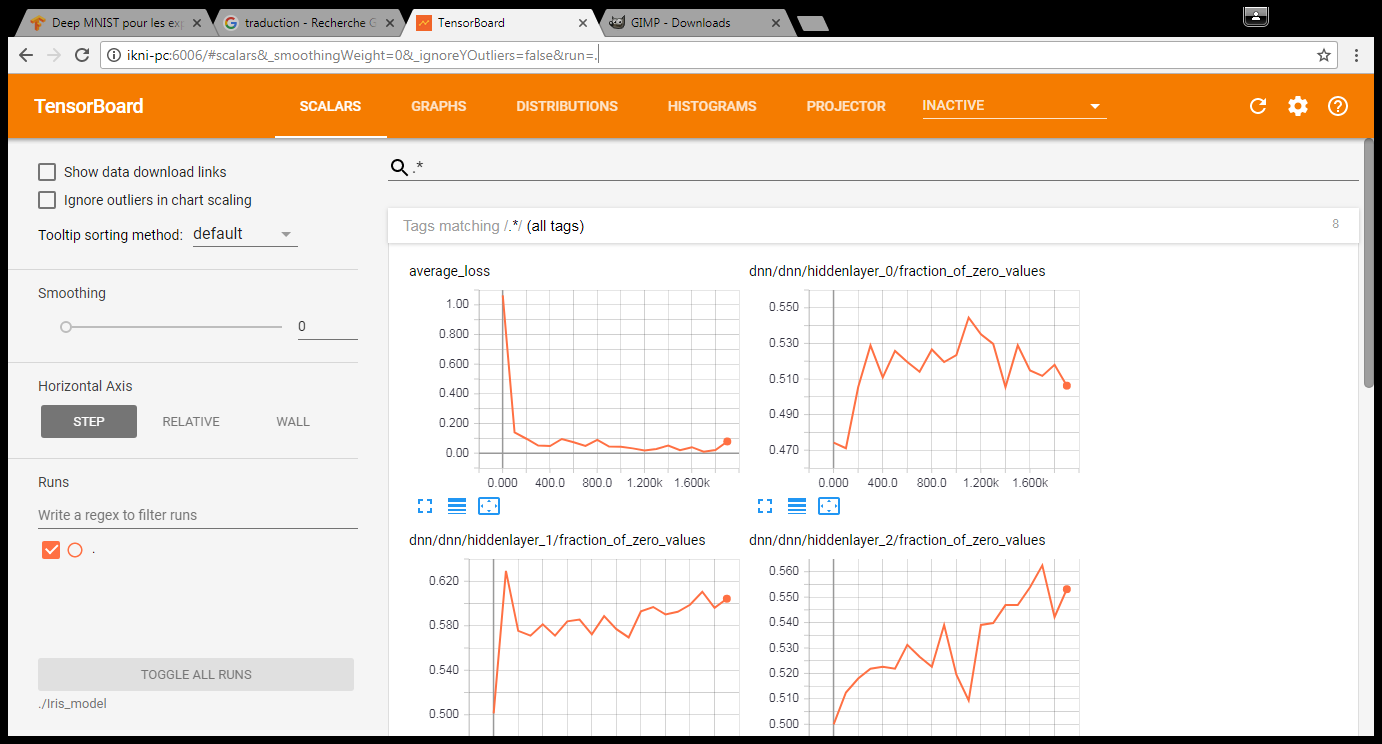
\includegraphics[width=16cm]{./figures/TensorBoardIrisDnn.png} 
\end{center}
\caption{Evolution des paramètres du réseau sur la base IRIS}
\end{figure}

\begin{figure}[H]

\begin{center}
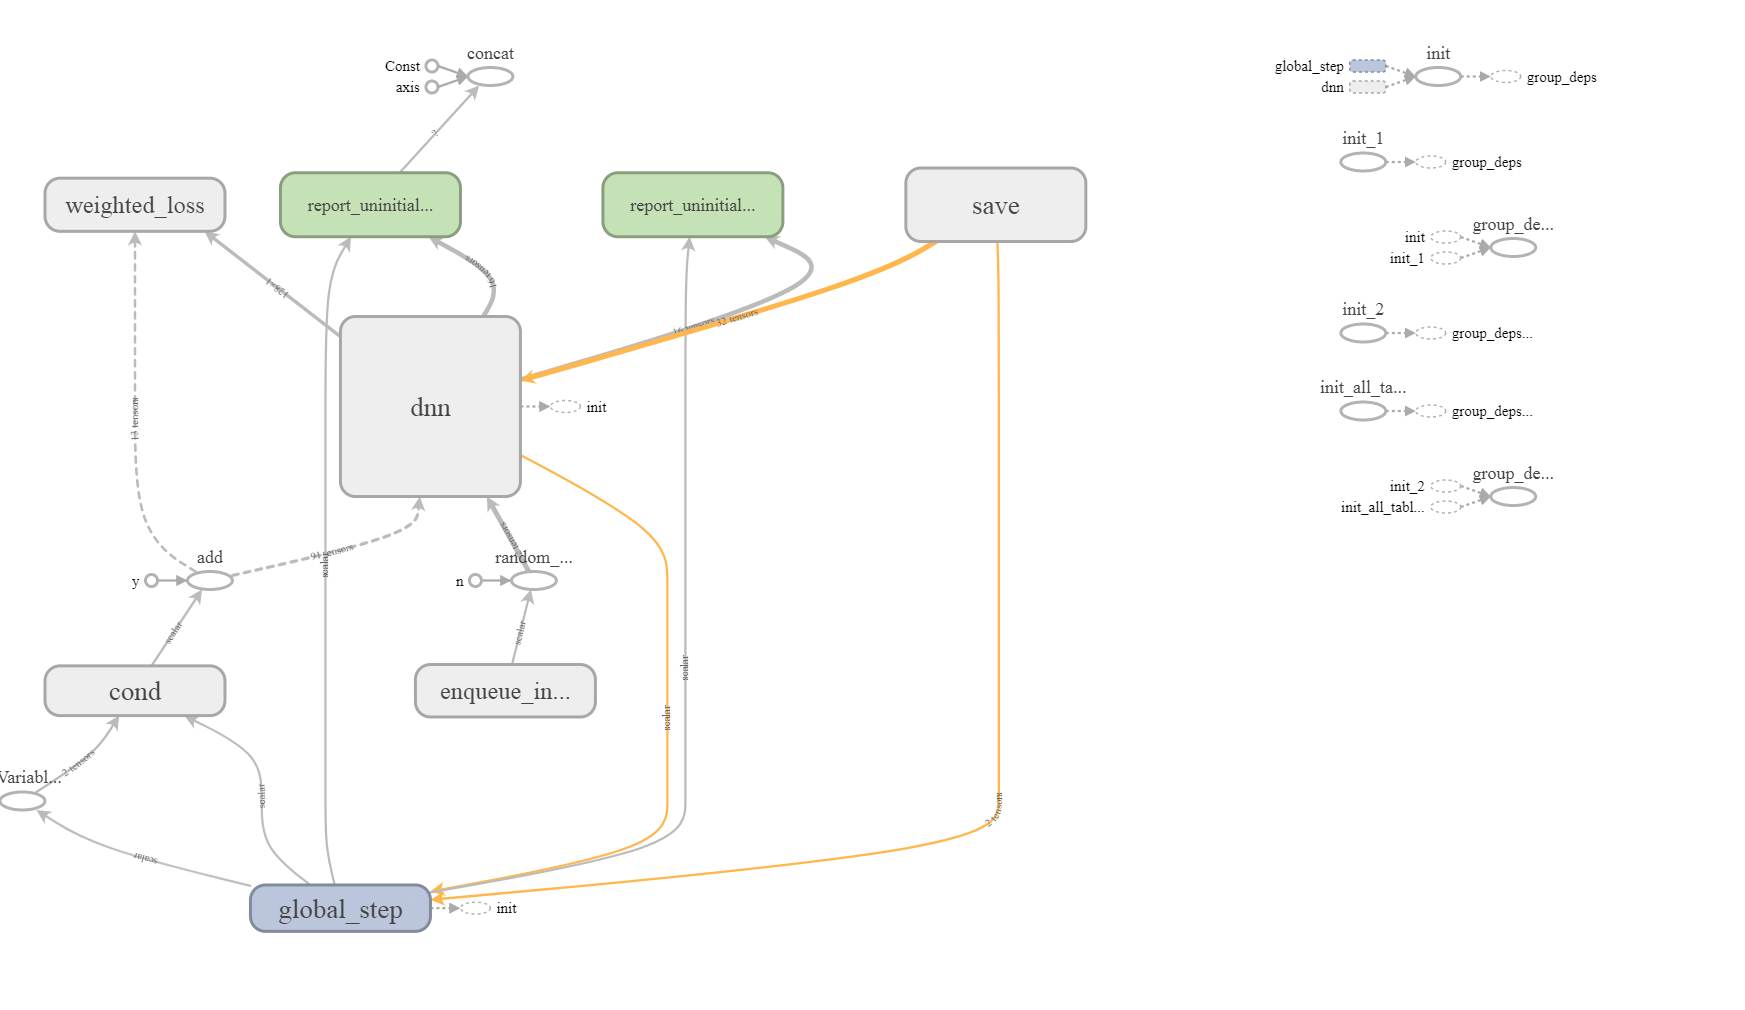
\includegraphics[width=10cm]{./figures/graphIrisDNN.png} 
\end{center}
\caption{Graphe de calcul du DNN utilisé sur la base IRIS}
\end{figure}

\subsection{Code du programme complet}

Notre programme est maintenant complet. Nous pouvons le trouver dans le fichier :\\
\verb+DNN/Documentation/TutosPython/Iris/irisDnnEstimatorComplet.py+

\lstinputlisting[style=generalFrame,backgroundcolor=\color{darkwhite}]{../../TutosPython/Iris/irisDnnEstimatorComplet.py}

\subsection{Sauvegarde et Chargement avec Estimator }
\label{sec:irisDnnSave}
Il s'agit maintenant de séparer notre programme en deux :
\begin{itemize}
\item Un programme qui apprend, évalue les performances et sauve le réseau
\item Un programme qui charge un réseau entraîné, et fait des prédictions.
\end{itemize}

Nous ne disposons plus d'un graphe, ni même d'une session. La procédure est donc totalement différente de ce qui a été vu dans la section~\ref{sec:irisMonocoucheSave}.

\subsubsection{Sauvegarde}
Les classifieurs de la classe Estimator savent sauvegarder leurs modèles grâce a la méthode \verb+export_savedmodel+.

Cependant cette méthode suppose la définition d'un modèle de service des données. 
Le modèle qui suit est fonctionnel et a été reconstitué à l'aide de fragments trouvés sur le web, sans que l'on ne comprenne vraiment tout ce qui s'y passe.

\begin{mypython}
def serving_input_receiver_fn():
  feature_spec = {'x': tf.FixedLenFeature([4],tf.float32)}
  serialized_tf_example = tf.placeholder(dtype=tf.string,
                                         shape=[None],
                                         name='input_tensors')
  receiver_tensors = {'inputs': serialized_tf_example}
  features = tf.parse_example(serialized_tf_example, feature_spec)
  return tf.estimator.export.ServingInputReceiver(features, receiver_tensors)
  
classifier.export_savedmodel('./savedNetworksEstimator', serving_input_receiver_fn)
\end{mypython}

Il faut noter que toutes les données sont sauvegardées dans un sous répertoire de celui que nous avons fourni. Le sous répertoire porte un nom correspondant à un timestamp obtenu lors de l'execution. notre programme complet renommera ce repertoire de sauvegarde en
\verb+./savedNetworksEstimator/lastSave+

Notons également la création d'un tenseur d'entrée pour les données qui porte le nom \verb+input_tensors+.

\subsubsection{Chargement}

Pour le chargement, nous procédons en deux étapes, peu claires.
\begin{mypython}
tf.saved_model.loader.load(sess, [tf.saved_model.tag_constants.SERVING], './savedNetworksEstimator/lastSave')

predictor= tf.contrib.predictor.from_saved_model('./savedNetworksEstimator/lastSave')
\end{mypython}

Enfin, nous récupérons le tenseur d'entrée de nos données :
\begin{mypython}
input_tensor=tf.get_default_graph().get_tensor_by_name("input_tensors:0")
\end{mypython}

Pour introduire un exemple dans le réseau, il faut préparer les données
\begin{mypython}
exemple = np.array([6.9, 3.2, 4.5, 1.5], dtype=np.float32)

model_input= tf.train.Example(features=tf.train.Features(feature={
					'x': tf.train.Feature(float_list=tf.train.FloatList(value=exemple))        
					}))
					
model_input=model_input.SerializeToString()				
\end{mypython}

Enfin, on peu calculer les prédictions.
\begin{mypython}
predictions= predictor({"inputs":[model_input]})
\end{mypython}

Cette prédiction est un dictionnaire dont la clef "scores" est ce qui nous intéresse :

\begin{mypython}
classe_id = np.argmax(predictions["scores"])
\end{mypython}

A ce stade, nous ne savons pas récupérer les probabilités de chaque classe. Nous travaillons encore sur ce point, mais le classifieur est fonctionnel.

\subsection{Programmes de sauvegarde et prédiction complets}
Dans ces programmes, nous avons ajouté quelques lignes pour paramétrer proprement les noms des fichiers et répertoires de sauvegarde et une procédure qui efface les répertoires de sauvegarde des modèles s'ils existent.

Voici le code du programme qui réalise l'apprentissage, contenu dans le fichier :\\
\verb+DNN/Documentation/TutosPython/Iris/irisDnnEstimatorTrain.py+

\lstinputlisting[style=generalFrame,backgroundcolor=\color{darkwhite}]{../../TutosPython/Iris/irisDnnEstimatorTrain.py}


Voici le code du programme qui réalise les prédictions, contenu dans le fichier :\\
\verb+DNN/Documentation/TutosPython/Iris/irisDnnEstimatorPredict.py+

\lstinputlisting[style=generalFrame,backgroundcolor=\color{darkwhite}]{../../TutosPython/Iris/irisDnnEstimatorPredict.py}

\section{Performances}
\label{secPerfIris}

Pour information, voici des performances standard obtenues sur la base Iris.
Monocouche :
\begin{myoutput}
Resultats en Apprentissage 0.98333335
Résultats en Généralisation 0.96666664
\end{myoutput}

Multicouches :
\begin{myoutput}
Resultats en Apprentissage 0.991667
Résultats en Généralisation 0.966667
\end{myoutput}

\chapter{bases MNIST et Fashion MNIST}
\section{La Base MNIST}

La base MNIST est bien connue, il s'agit de reconnaitre des chiffres (10 classes), a partir d'images de 28x28 pixels, que dans un premier temps nous transformerons en un vecteur de 784 valeurs.

\subsection{Lecture des données}
\label{secGetMnist}
Lecture des données : Nous importons un module permettant de récupérer la base MNIST, puis on demande à ce module de lire les données. Si elles ne sont pas présentes, il va les télécharger sur le site de MNIST 
(\verb+http://yann.lecun.com/exdb/mnist/+)

\begin{mypython}
from tensorflow.examples.tutorials.mnist import input_data
mnist = input_data.read_data_sets("MNIST_data/")
\end{mypython}

L'objet contenant nos données permet l'accès aux données d'apprentissage dans \verb+mnist.train.images+ et \verb+mnist.train.labels+.
Les données de généralisations sont accessible via 
\verb+mnist.test.images+ et \verb+mnist.test.labels+.


Lorsque nous voudrons faire de la prédiction, nous partirons d'une image quelconque, qu'il faudra préparer (transformer en image 28x28, inverser le contraste...) On pourra le faire comme suit :
\begin{mypython}
imageFilename = 'images/bidon.jpg'
imageGray = Image.open(imageFilename).resize((28,28)).convert('L')
imageInvert =  PIL.ImageOps.invert(imageGray)

#imageInvert.save('temp.bmp')


# conversion en vecteur
a = np.array(imageInvert)
flat_arr = a.reshape((1, 784))
\end{mypython}
Ce dernier vecteur pourra être introduit dans les réseaux.


\subsection{Mnist : Réseau monocouche boite blanche}

\subsubsection{Construction du modèle}
\label{secMnistDnnBuild}

On utilisera ici un modèle purement linéaire contenant une couche de 10 neurones (c'est la couche de sortie) tout à fait semblable à celui de la base Iris vu dans la section~\ref{sec:irisMonocoucheBuild}. Simplement, il y a maintenant 10 neurones et 784 entrées.
 
\begin{mypython}
# entrées
x = tf.placeholder(tf.float32, [None, 784])

# sorties voulues
y_ = tf.placeholder(tf.float32, [None, 10])

# Le modèle
W = tf.Variable(tf.zeros([784, 10]))
b = tf.Variable(tf.zeros([10]))

# sorties calcules 
score = tf.matmul(x, W) + b
\end{mypython}

Les calculs d'entropie croisée et de précision sont ceux vu dans la section~\ref{sec:irisMonocoucheBuild}

\subsubsection{Lancement des calculs}
\label{secMnistDnnRun}

L'apprentissage est très semblable à celui que nous avons fait pour la base Iris, a ceci prêt que nous tirons profit de l'objet mnist qui permet de faire des batch de 100 exemples.

Ici, nous proposons un apprentissage en 1000 passes sur 100 exemples tirés au sort.

\begin{mypython}
# Apprentissage
for i in range(1000):
  batch_xs, batch_ys = mnist.train.next_batch(100)
  sess.run(train_step, feed_dict={x: batch_xs, y_: batch_ys})
\end{mypython}

L'évaluation est classique. Par exemple, en généralisation :
\begin{mypython}
print("Résultats en Généralisation", sess.run(accuracy, feed_dict={x: mnist.test.images, 	y_: mnist.test.labels}))
\end{mypython}

Pour la prédiction, il faudra lire une image, la transformer en vecteur de taille 784 comme on l'a vu dans la section~\ref{secGetMnist}
Ce dernier vecteur est alors introduit dans le réseau pour prédiction

\begin{mypython}
print("\nJe pense que c'est un ", sess.run(classe, {x: flat_arr}))
\end{mypython}

\subsubsection{Codes complets }
Le code complet, incluant des instructions de mise en forme pour TensorBoard est le suivant. Ce code est contenu dans le fichier :\\
\verb+DNN/Documentation/TutosPython/Mnist/mnistMonocoucheComplet.py+

\lstinputlisting[style=generalFrame,backgroundcolor=\color{darkwhite}]{../../TutosPython/Mnist/mnistMonocoucheComplet.py}

Ci dessous, le code complet du programme en charge de l'apprentissage et de la sauvegarde du modèle. Ce code est contenu dans le fichier :\\
\verb+DNN/Documentation/TutosPython/Mnist/mnistMonocoucheTrain.py+

\lstinputlisting[style=generalFrame,backgroundcolor=\color{darkwhite}]{../../TutosPython/Mnist/mnistMonocoucheTrain.py}

Enfin, voici le code complet du programme en charge du chargement d'un réseau et de la réalisation des prédictions. Ce code est contenu dans le fichier :\\
\verb+DNN/Documentation/TutosPython/Mnist/mnistMonocouchePredict.py+

\lstinputlisting[style=generalFrame,backgroundcolor=\color{darkwhite}]{../../TutosPython/Mnist/mnistMonocoucheTrain.py}


\subsection{Mnist : Réseau multicouches boite noire}
\label{secMnistMulti}

Le lecteur peut se référer à la section~\ref{sec:irisMulticoucheBuild} pour la construction d'un réseau multicouche avec Estimator.
Les principes ayant été vu, nous nous bornerons a donner le code complet des trois programmes : Complet, Train, Predict.

\subsubsection{Codes complets }
Le code complet, incluant des instructions de mise en forme pour TensorBoard est le suivant. Ce code est contenu dans le fichier :\\
\verb+DNN/Documentation/TutosPython/Mnist/mnistDnnEstimatorComplet.py+

\lstinputlisting[style=generalFrame,backgroundcolor=\color{darkwhite}]{../../TutosPython/Mnist/mnistDnnEstimatorComplet.py}

Ci dessous, le code complet du programme en charge de l'apprentissage et de la sauvegarde du modèle. Ce code est contenu dans le fichier :\\
\verb+DNN/Documentation/TutosPython/Mnist/mnistDnnEstimatorTrain.py+

\lstinputlisting[style=generalFrame,backgroundcolor=\color{darkwhite}]{../../TutosPython/Mnist/mnistDnnEstimatorTrain.py}

Enfin, voici le code complet du programme en charge du chargement d'un réseau et de la réalisation des prédictions. Ce code est contenu dans le fichier :\\
\verb+DNN/Documentation/TutosPython/Mnist/mnistDnnEstimatorPredict.py+

\lstinputlisting[style=generalFrame,backgroundcolor=\color{darkwhite}]{../../TutosPython/Mnist/mnistDnnEstimatorTrain.py}

\subsection{Performances}
\label{secPerfMnist}

Pour information, voici des performances standard obtenues sur la base MNIST.
Monocouche :
\begin{myoutput}
Résultats en Apprentissage 0.91827273
Résultats en Généralisation 0.9178
\end{myoutput}

Multicouches :
\begin{myoutput}
Resultats en Apprentissage 0.98333335
Résultats en Généralisation 0.96666664
\end{myoutput}

\section{La base Fashion MNIST}

La base Fashion MNIST ressemble beaucoup à la base MNIST :
\begin{itemize}
\item Même nombre d'entrées
\item Même nombre de classes
\item Même nombre d'exemples
\item Même noms de fichiers
\end{itemize}

\subsection{Lecture des données}
\label{secGetFmnist}

De ce fait, nous pouvons utiliser les mêmes procédures pour charger les exemples que celle utilisées pour MNIST. Ces procédures font partie du module exemple de tensorflow que l'on charge comme suit :
\begin{mypython}
from tensorflow.examples.tutorials.mnist import input_data
\end{mypython}
La seule modification effective consiste a spécifier le répertoire ou l'on trouve les fichiers de Fashion MNIST :
\begin{mypython}
# Import data
fashionMnist = input_data.read_data_sets('./FM_DATA/')
\end{mypython}
C'est cet objet \verb+fashionMnist+ qui fournira les données et les labels lors de l'entrainement et de l'évaluation.

\textbf{ATTENTION :} Nous utilisons içi un module conçu pour MNIST pour lire les données de Fashion MNIST. Conformément à ce qui a été dit dans la section~\ref{secGetMnist}, si le répertoire \verb+./FM_DATA/+ est vide ou n'existe pas, ce module va télécharger la base MNIST dedans !
Le téléchargement de Fashion MNIST doit donc être fait manuellement, depuis\\
\verb+https://github.com/zalandoresearch/fashion-mnist/+.

\subsection{Fmnist : Réseau monocouche boite blanche}
\label{secFashionMnistMono}
Compte tenu de ce qui a été dit plus haut, le code est quasiment le même que dans le cas de MNIST vu dans la section \ref{secMnistMono}. 
Voici donc le code complet du programme. Ce code est contenu dans le fichier :\\
\verb+DNN/Documentation/TutosPython/FashionMNIST/fmnistMonocoucheComplet.py+

\lstinputlisting[style=generalFrame,backgroundcolor=\color{darkwhite}]{../../TutosPython/FashionMNIST/fmnistMonocoucheComplet.py}

\subsection{Fmnist : Réseau multicouche boite noire}
\label{secFashionMnistMulti}
Compte tenu de ce qui a été dit plus haut, le code est quasiment le même que dans le cas de MNIST vu dans la section \ref{secMnistMulti}. 
Voici donc le code complet du programme. Ce code est contenu dans le fichier :\\
\verb+DNN/Documentation/TutosPython/FashionMNIST/fmnistDnnEstimatorComplet.py+

\lstinputlisting[style=generalFrame,backgroundcolor=\color{darkwhite}]{../../TutosPython/FashionMNIST/fmnistDnnEstimatorComplet.py}


\subsection{Performances}
\label{secPerfFMnist}

Pour information, voici des performances standard obtenues sur la base Fashion MNIST.
Monocouche :
\begin{myoutput}
Resultats en Apprentissage 0.79394543
Résultats en Généralisation 0.7783
\end{myoutput}

Multicouches :
\begin{myoutput}
Resultats en Apprentissage 0.889000
Résultats en Généralisation 0.868800
\end{myoutput}

On peut noter la baisse de performances par rapport à ce qui était obtenu avec la base MNIST dans la section ~\ref{secPerfMnist}.

\end{document}
